% Letter-local standalone mirroring figures/fig_hca_standalone.tex,
% but using downsampled HCA PNGs (1000 px) from ../shared/ to keep
% the response-letter PDF compact.
% Compile: pdflatex fig_r2_3.tex
\documentclass[border=5pt]{standalone}
\usepackage{tikz}
\usetikzlibrary{arrows.meta, calc}
\usepackage{amsmath}
\usepackage{graphicx}
\graphicspath{{../shared/}}

\begin{document}
\begin{tikzpicture}[
  every node/.style={font=\small},
  dimarr/.style={{Stealth[length=3pt]}-{Stealth[length=3pt]}, thin, black!60},
  lbl/.style={font=\footnotesize},
  stress/.style={-{Stealth[length=4pt]}, thick, red!70!black},
  stressp/.style={-{Stealth[length=4pt]}, thick, blue!70!black},
]
  % ==================== (a) Perspective view ====================
  \node[anchor=south west, inner sep=0] (imgA) at (0,0)
    {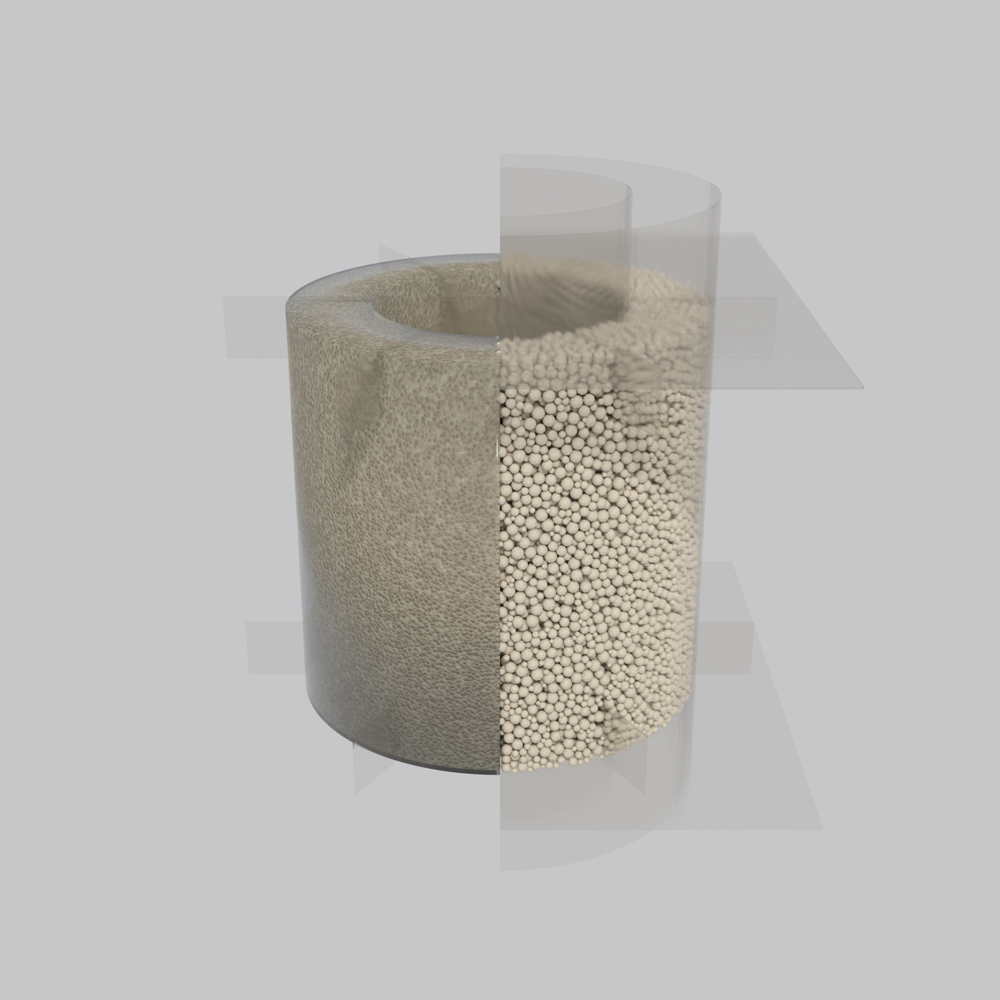
\includegraphics[width=8cm]{hca_final_perspective_small.png}};
  \begin{scope}[
    x={(imgA.south east)},
    y={(imgA.north west)},
  ]
    % --- Headers ---
    \node[font=\normalsize\bfseries] at (0.27, 0.96) {Laboratory};
    \node[font=\normalsize\bfseries] at (0.70, 0.96) {DEM};

    % === Lab outer wall (left silhouette) ===
    \coordinate (wallLBot) at (0.3, 0.18);
    \coordinate (wallLTop) at (0.27, 0.8);
    \pgfmathsetmacro{\poLen}{0.06} % arrow length (fraction of wall length)
    \foreach \t/\idx in {0.20/1, 0.40/2, 0.60/3, 0.80/4} {
      \pgfmathsetmacro{\fac}{\poLen/(1-\t)}
      \coordinate (poTail\idx) at ($(wallLBot)!\t!(wallLTop)!\fac!90:(wallLTop)$);
      \draw[stress]
        (poTail\idx) -- ($(wallLBot)!\t!(wallLTop)$);
    }
    % connect tails (pressure baseline)
    \draw[thin, red!70!black] (poTail1) -- (poTail2) -- (poTail3) -- (poTail4);
    \node[lbl, red!70!black, left] at
      ($(wallLBot)!0.50!(wallLTop)!{0.06/0.5}!90:(wallLTop)$) {$p_o$};

    % === Lab top surface (p_z) — vertical arrows along elliptical arc ===
    \pgfmathsetmacro{\pzH}{0.035}          % arrow length
    \pgfmathsetmacro{\topCxL}{0.5}       % ellipse center x
    \pgfmathsetmacro{\topCyL}{0.7}       % ellipse center y
    \pgfmathsetmacro{\topRxL}{0.18}       % x semi-axis
    \pgfmathsetmacro{\topRyL}{0.05}      % y semi-axis (perspective foreshortening)
    \foreach \ang in {105, 125, 145, 165, 185, 205, 225, 255} {
      \pgfmathsetmacro{\px}{\topCxL + \topRxL*cos(\ang)}
      \pgfmathsetmacro{\py}{\topCyL + \topRyL*sin(\ang)}
      \draw[stress] (\px, {\py + \pzH}) -- (\px, \py);
    }
    % baseline arc (connecting tails)
    \draw[thin, red!70!black]
      plot[smooth, samples=30, domain=105:255]
        ({\topCxL + \topRxL*cos(\x)}, {\topCyL + \topRyL*sin(\x) + \pzH});
    \node[lbl, red!70!black, above left] at ({\topCxL - 0.05}, {\topCyL + \topRyL*sin(270) + \pzH + 0.1}) {$p_z$};

    % === u label ===
    %\node[lbl, cyan!50!blue, font=\footnotesize\itshape] at (0.28, 0.22) {$u$};

    % === DEM outer wall (right silhouette) ===
    \coordinate (wallRBot) at (0.7, 0.18);
    \coordinate (wallRTop) at (0.73, 0.8);
    \pgfmathsetmacro{\poLenR}{0.06}
    \foreach \t/\idx in {0.20/1, 0.40/2, 0.60/3, 0.80/4} {
      \pgfmathsetmacro{\facR}{\poLenR/(1-\t)}
      \coordinate (poTailR\idx) at ($(wallRBot)!\t!(wallRTop)!\facR!-90:(wallRTop)$);
      \draw[stressp]
        (poTailR\idx) -- ($(wallRBot)!\t!(wallRTop)$);
    }
    % connect tails (pressure baseline)
    \draw[thin, blue!70!black] (poTailR1) -- (poTailR2) -- (poTailR3) -- (poTailR4);
    \node[lbl, blue!70!black, right] at
      ($(wallRBot)!0.50!(wallRTop)!{0.06/0.5}!-90:(wallRTop)$) {$p_o^\prime$};

    % === DEM top surface (p_z') — vertical arrows along elliptical arc ===
    \pgfmathsetmacro{\pzHR}{0.035}
    \pgfmathsetmacro{\topCxR}{0.5}       % ellipse center x (same specimen center)
    \pgfmathsetmacro{\topCyR}{0.7}       % ellipse center y
    \pgfmathsetmacro{\topRxR}{0.18}      % x semi-axis
    \pgfmathsetmacro{\topRyR}{0.05}      % y semi-axis
    \foreach \ang in {-75, -55, -35, -15, 15, 35, 55, 75} {
      \pgfmathsetmacro{\px}{\topCxR + \topRxR*cos(\ang)}
      \pgfmathsetmacro{\py}{\topCyR + \topRyR*sin(\ang)}
      \draw[stressp] (\px, {\py + \pzHR}) -- (\px, \py);
    }
    % baseline arc (connecting tails)
    \draw[thin, blue!70!black]
      plot[smooth, samples=30, domain=-75:75]
        ({\topCxR + \topRxR*cos(\x)}, {\topCyR + \topRyR*sin(\x) + \pzHR});
    \node[lbl, blue!70!black, above right] at ({\topCxR + 0.05}, {\topCyR + \topRyR*sin(270) + \pzHR + 0.1}) {$p_z^\prime$};

    % === H dimension ===
    \draw[dimarr] (0.86, 0.32) -- (0.86, 0.70);
    \node[lbl, black!60, right] at (0.88, 0.5) {$H$};

    % --- DEBUG: grid overlay (uncomment to help with positioning) ---
    % \draw[help lines, step=0.1, gray!30] (0,0) grid (1,1);
    % \foreach \x in {0.0, 0.1, ..., 1.0} {
    %   \node[font=\tiny, gray] at (\x, -0.02) {\x};
    % }
    % \foreach \y in {0.0, 0.1, ..., 1.0} {
    %   \node[font=\tiny, gray] at (-0.03, \y) {\y};
    % }
  \end{scope}

  % ==================== (b) Top-down view ====================
  \node[anchor=south west, inner sep=0] (imgB) at (8.5,0)
    {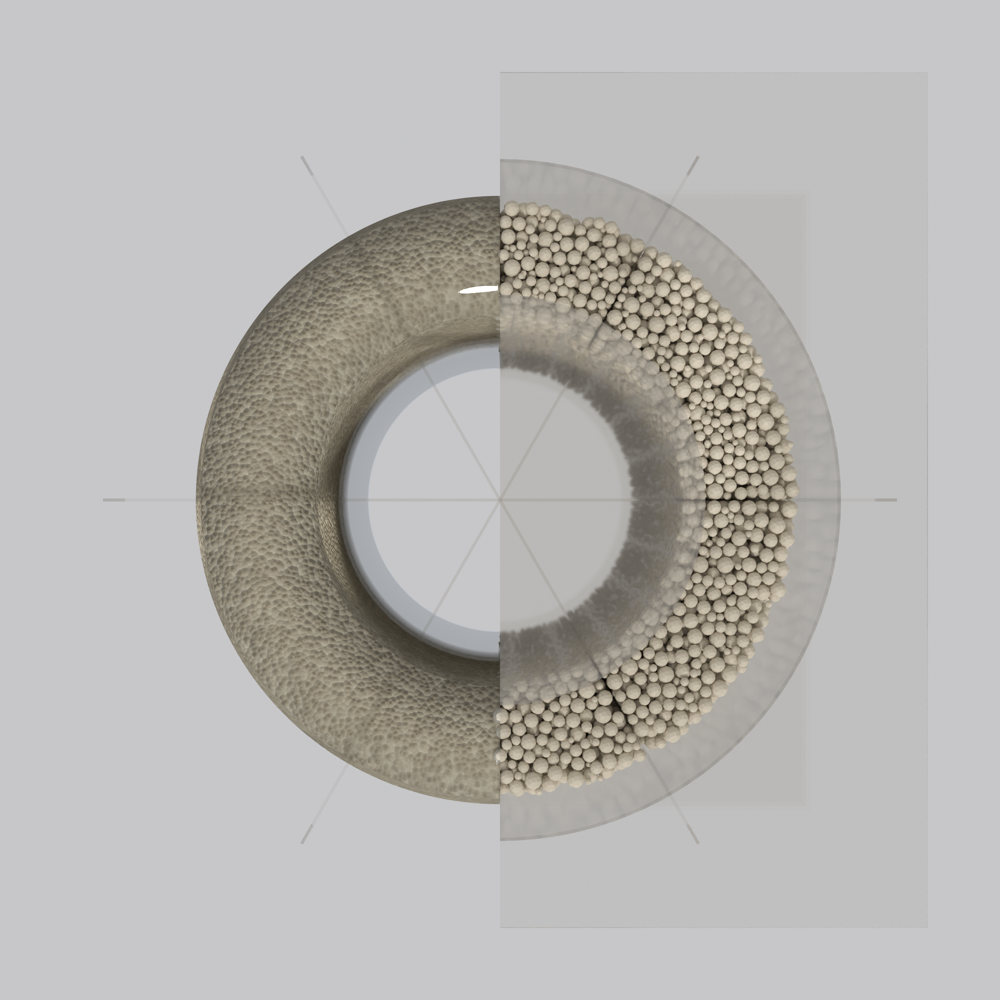
\includegraphics[width=8cm]{hca_final_topdown_small.png}};
  \begin{scope}[
    x={($(imgB.south east)-(imgB.south west)$)},
    y={($(imgB.north west)-(imgB.south west)$)},
    shift={(imgB.south west)},
  ]
    % --- Headers ---
    \node[font=\normalsize\bfseries] at (0.25, 0.96) {Laboratory};
    \node[font=\normalsize\bfseries] at (0.75, 0.96) {DEM};

    % Annulus center
    \coordinate (C) at (0.50, 0.50);

    % === Lab outer wall p_o ===
    \pgfmathsetmacro{\poTailR}{0.39}     % tail radius (outer)
    \pgfmathsetmacro{\poTailRy}{0.38}
    \pgfmathsetmacro{\poHeadR}{0.34}     % head radius (on wall)
    \pgfmathsetmacro{\poHeadRy}{0.33}
    \foreach \ang in {110, 130, 150, 170, 190, 210, 230, 250} {
      \pgfmathsetmacro{\ox}{0.50 + \poTailR*cos(\ang)}
      \pgfmathsetmacro{\oy}{0.50 + \poTailRy*sin(\ang)}
      \pgfmathsetmacro{\ix}{0.50 + \poHeadR*cos(\ang)}
      \pgfmathsetmacro{\iy}{0.50 + \poHeadRy*sin(\ang)}
      \draw[stress] (\ox, \oy) -- (\ix, \iy);
    }
    % connect tails (pressure baseline arc)
    \draw[thin, red!70!black]
      plot[smooth, samples=30, domain=110:250]
        ({0.50 + \poTailR*cos(\x)}, {0.50 + \poTailRy*sin(\x)});
    \node[lbl, red!70!black] at
      ({0.50 + 0.44*cos(180)}, {0.50 + 0.43*sin(180)}) {$p_o$};

    % === Lab inner wall p_i ===
    \pgfmathsetmacro{\piTailR}{0.12}     % tail radius (inner, toward center)
    \pgfmathsetmacro{\piTailRy}{0.11}
    \pgfmathsetmacro{\piHeadR}{0.17}     % head radius (on wall)
    \pgfmathsetmacro{\piHeadRy}{0.16}
    \foreach \ang in {110, 130, 150, 170, 190, 210, 230, 250} {
      \pgfmathsetmacro{\ix}{0.50 + \piTailR*cos(\ang)}
      \pgfmathsetmacro{\iy}{0.50 + \piTailRy*sin(\ang)}
      \pgfmathsetmacro{\ox}{0.50 + \piHeadR*cos(\ang)}
      \pgfmathsetmacro{\oy}{0.50 + \piHeadRy*sin(\ang)}
      \draw[stress] (\ix, \iy) -- (\ox, \oy);
    }
    % connect tails (pressure baseline arc)
    \draw[thin, red!70!black]
      plot[smooth, samples=30, domain=110:250]
        ({0.50 + \piTailR*cos(\x)}, {0.50 + \piTailRy*sin(\x)});
    \node[lbl, red!70!black] at
      ({0.50 + 0.07*cos(180)}, {0.50 + 0.06*sin(180)}) {$p_i$};

    % === DEM outer wall p_o' ===
    \pgfmathsetmacro{\poTailRR}{0.39}
    \pgfmathsetmacro{\poTailRRy}{0.38}
    \pgfmathsetmacro{\poHeadRR}{0.34}
    \pgfmathsetmacro{\poHeadRRy}{0.33}
    \foreach \ang in {-70, -50, -30, -10, 10, 30, 50, 70} {
      \pgfmathsetmacro{\ox}{0.50 + \poTailRR*cos(\ang)}
      \pgfmathsetmacro{\oy}{0.50 + \poTailRRy*sin(\ang)}
      \pgfmathsetmacro{\ix}{0.50 + \poHeadRR*cos(\ang)}
      \pgfmathsetmacro{\iy}{0.50 + \poHeadRRy*sin(\ang)}
      \draw[stressp] (\ox, \oy) -- (\ix, \iy);
    }
    % connect tails (pressure baseline arc)
    \draw[thin, blue!70!black]
      plot[smooth, samples=30, domain=-70:70]
        ({0.50 + \poTailRR*cos(\x)}, {0.50 + \poTailRRy*sin(\x)});
    \node[lbl, blue!70!black] at
      ({0.50 + 0.44*cos(0)}, {0.50 + 0.43*sin(0)}) {$p_o^\prime$};

    % === DEM inner wall p_i' ===
    \pgfmathsetmacro{\piTailRR}{0.12}
    \pgfmathsetmacro{\piTailRRy}{0.11}
    \pgfmathsetmacro{\piHeadRR}{0.17}
    \pgfmathsetmacro{\piHeadRRy}{0.16}
    \foreach \ang in {-70, -50, -30, -10, 10, 30, 50, 70} {
      \pgfmathsetmacro{\ix}{0.50 + \piTailRR*cos(\ang)}
      \pgfmathsetmacro{\iy}{0.50 + \piTailRRy*sin(\ang)}
      \pgfmathsetmacro{\ox}{0.50 + \piHeadRR*cos(\ang)}
      \pgfmathsetmacro{\oy}{0.50 + \piHeadRRy*sin(\ang)}
      \draw[stressp] (\ix, \iy) -- (\ox, \oy);
    }
    % connect tails (pressure baseline arc)
    \draw[thin, blue!70!black]
      plot[smooth, samples=30, domain=-70:70]
        ({0.50 + \piTailRR*cos(\x)}, {0.50 + \piTailRRy*sin(\x)});
    \node[lbl, blue!70!black] at
      ({0.50 + 0.07*cos(0)}, {0.50 + 0.06*sin(0)}) {$p_i^\prime$};

    % === Dimensions ===
    \draw[dimarr] (0.50, 0.12) -- (0.68, 0.12);
    \node[lbl, black!60, below] at (0.59, 0.13) {$r$};
    \draw[dimarr] (0.50, 0.07) -- (0.786, 0.07);
    \node[lbl, black!60, below] at (0.643, 0.06) {$R$};

    % === T: torque ===
    \pgfmathsetmacro{\tRx}{0.36}
    \pgfmathsetmacro{\tRy}{0.36}
    \draw[-{Stealth[length=4pt]}, thick, black!70]
      plot[smooth, samples=20, domain=80:100]
        ({0.50 + \tRx*cos(\x)}, {0.50 + \tRy*sin(\x)});
    \node[lbl, black!70] at (0.50, 0.88) {$T$};

    % --- DEBUG: grid overlay (uncomment to help with positioning) ---
    % \draw[help lines, step=0.1, gray!30] (0,0) grid (1,1);
    % \foreach \x in {0.0, 0.1, ..., 1.0} {
    %   \node[font=\tiny, gray] at (\x, -0.02) {\x};
    % }
    % \foreach \y in {0.0, 0.1, ..., 1.0} {
    %   \node[font=\tiny, gray] at (-0.03, \y) {\y};
    % }
  \end{scope}
\end{tikzpicture}
\end{document}
